\documentclass[fontsize=11pt]{article}
\usepackage{amsmath}
\usepackage[utf8]{inputenc}
\usepackage[margin=0.75in]{geometry}
\usepackage{graphicx}
\title{CSC111 Project Proposal: OpenMetroGuide}
\author{Ansh Jain, Nikhil Sreekumar, Sidharth Sachdev}
\date{Tuesday, March 16, 2021}

\begin{document}
    \maketitle

    \section*{Problem Description and Research Question}

    Being a tourist or a non-public-transport user can be difficult especially when trying to figure out the optimum path from your current location to your destination. Looking at the transit maps on the metro lines might provide a general idea of the location of stations, but understanding the best possible routes to get from one location to another easily requires experience, especially as the metro grids get complex. Even though cities like Toronto and Dubai do not have a complex transit map, it can still be troublesome for a first-time user. Cities like London and New York have a web of train stations and tracks. Navigating through these paths can be challenging not only for tourists but also for residents.\newline


    \begin{center}
        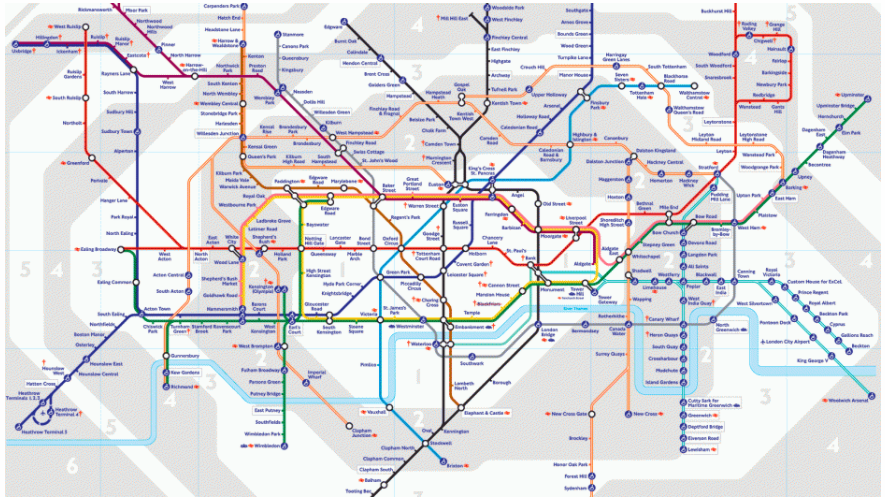
\includegraphics[width = 14cm]{London Transit Map.png}\newline
        London Underground is an example of an extremely complex metro grid.
    \end{center}

    \textbf{Goal 1: Our project helps its users visualize the best possible path between two stations, based on their preference for a faster or a cheaper route}.\newline

    While navigating the map as mentioned above is a complex task, making sure that the metro map is up-to-date and notifies users of real-time situations is a problem as well. The secondary objective of our project is to enable map administrators to make frequent changes for the maintenance of these metro maps. We do so by providing a set of the most common utilities that would be required by maintainers irrespective of the city that they are concerned with. It is clear that there are certain aspects of updating map in real-time (Train delays, stations under maintenance etc.) that are issues all metros would have to deal with. OpenMetroGuide creates an open standard based on how the metro stations are maintained and read.\newline


    \textbf{Goal 2:
    Our project can be a pioneer in using this open standard to make real-time maintenance and use of online metro maps world-wide easier.
    }\newline

    \subsubsection{TA's suggestion}
    As per the TA's suggestion to change the title of the project to be a bit more specific, we renamed it to $\dots$\\
    \textbf{TODO: ADD NEW NAME.}\\
    We also used the suggestion to implement Hamiltonian graphs in order to check whether the map is connected at all times. If not, then the application displays a message indicating that the map isn't connected.
    \section*{Data-sets Description}
    There are no prior datasets that need to be downloaded or are present in the program. Instead, the user is responsible for reading or writing into the local database depending on the users privileges (Admin or User). There are through instructions that guide the user before viewing/editing of the maps can begin. This includes error messages if the local database is empty. Using these navigation steps at the start and the creation of metro maps following the steps, the local database will be populated.

    \section*{Computational Plan}
%This application can be accessed by two types of users. One is the map administrator/maintainer and the other is the client using the application for travel information.
    Our project represents the metro transit map of a city/region as a graph and utilize it by displaying the best possible shortest or cheapest route. It can be used by 2 types of users, the administrator and the client. The administrator has the ability to modify the map and save the result into a database. The client utilizes the map for navigation purposes to serve his need of travel by pursuing the cheapest or the shortest path as per his wish. Every user will be able to choose whether he is a client or an administrator based on the option they choose. Based on the choice made, a corresponding \textbf{Admin(User)} or \texttt{Client(User)} is created and the respective methods are called. Both the client and the admin are subclasses of abstract user class.


    \subsection*{Creating the map}
    The map administrator will be able to develop the map of that region such as Dubai or Toronto and have the option to edit it.
    These editing options include:
    \begin{itemize}
        \item Adding a station
        \item Adding a track
        \item Removing a station
        \item Removing the track
    \end{itemize}
    Since the map is a graph, stations represents its vertices and tracks represents the edges. \\
    This will be implemented using the \texttt{pygame} package where the screen will be converted into small grids (similar to the linked list assignment but a lot smaller) for the ease of the user. The administrator will be able to draw tracks in these lines and add station on the square intersections of the grid(not the diagonal intersections). \\
    Three of the main pygame methods that are used to represent the lines, circles, and, rectangles are:
    \begin{itemize}
        \item \texttt{pygame.draw.line()}
        \item \texttt{pygame.draw.circle()}
        \item \texttt{pygame.draw.rect()}
    \end{itemize}
    Whenever the administrator adds a station to the map, he is presented with a dialogue box asking information such as the \textit{name of the station} and its \textit{zone}. Using the color palette on the right side of the screen, the administrator can select the color of the track to be drawn.\\
    The selecting and clicking on the map has been performed under the \texttt{handle\_mouse\_click()} function using the \texttt{pygame} class \texttt{pygame.event} specifically \texttt{pygame.event.MOUSEBUTTONDOWN}. Using the co-ordinates of the click of the mouse, we can determine what is being selected. In the case of circles, this is performed by comparing the Cartesian distance between the click and the center of the circle with the help of its radius. In the case of rectangles, we use a method of the \texttt{pygame.Rect()} object which is \texttt{collidepoint()}. A similar concept has been used to represent the information of a created station when hovering over it on the map using the function \texttt{pygame.mouse.get\_pos()}.\\
    \\
    Once the map has been created and the user exits the window, the map is automatically saved onto the database. When reloading the application, the name of the cities who's map has been created is displayed and the admin can either choose an existing map to further edit it or create a new map altogether.

    \subsection*{Implementing Datasets}
	The storage of data in the application has the following plan:
	
	\begin{enumerate}
		\item The Admin, after having created the map, automatically saves his creation (or edits if the map was pre-existing).
		
		\item The User will be able to access the cities the currently have a plan associated with them, and can choose the city for which the optimization is desired.
		
		\item The Admin also has access to previously created maps, should it be required to edit an existing plan.
	\end{enumerate}

	As seen above, the read/write queries made is quite frequent. Moreover, there are several graphs, of which nodes have several attributes. Thus, it would not be ideal to use a csv file for the storage and retrieval of such data, due to the inefficiency and complexity. Therefore, a lightweight RDBMS alternative was required, and the storage was instead performed with SQLite using the python library \texttt{sqlite3}.
	
	 There are two tables. The first table represents the nodes of the metro maps, while the second represents the relations between each node with others. The first table had columns representing the cities, and every other attribute represented the attributes part of the \texttt{Node} object is the maps. This is similarly true for the connections table. This extra cities column was necessary so as to perform queries of adding and deleting information on the same map. This was done by filtering the database on the basis of city name.
	 
	 Since each read/write occurred together and was localized for each map,  no minor updates were needed to be taken care of. Hence, there was no usage of a primary and foreign key to link the two tables. However, it should be noted that this implementation is much more efficient, as the task of ensuring uniqueness had to be dealt with in \texttt{python} by OpenMetroGuide. 

    \subsection*{Implementing the map}
    Just the administrator, the user will have the option to choose from one of the existing maps(they won't be able to create a new map, obviously). The user interface will consist of an interactive map created by the admin. A complete map of the metro will be displayed on the screen (reading from local database) and the user will be able to choose a starting station and a final destination station by selecting the stations on the map. A right click will be used to select the destination station and the left click will will indicate the starting station.The selected station will indicate whether they are the starting station or the destination station when selected.\\
    They will also be able to choose whether they want a time-optimized or a cost-optimized route which will be represented by 2 images on the right side of the map. The images were inserted using the \textbf{pygame.image.load()} function. The selection is done with the same concept as described above in the case of creating the map.\\
    Based on these inputs, our application will provide the best route using the A* search algorithm.\\
    \\
    We will be using a weighted graph, where the vertices are train stations (with an attribute for direct distance from the destination) and the weighted edges represent the path between adjacent stations with a length attribute. \\
    \\
    Dijkstra's algorithm is an optimization algorithm to find "the shortest paths between nodes in a graph". This algorithm will be implemented using a priority queue based on the above-mentioned heuristics. The priority queue will be a list of stations ordered based on the cumulated edge lengths combined with either distance from destination or cost. All (unvisited) nodes are initially marked at a distance of infinity from the starting node (which is passed in as the current node). The shortest route will be calculated by prioritizing the distance and edge length whereas the cheapest route will be calculated by giving cost and edge length more importance. Each of the current node's neighbors (except the previously visited ones in the current recursion stack) is given a numeric value based on the weighted edges. Once the destination station is reached, we retrace the stations using recursion till the start station which will be the optimum route. \textbf{The A* search algorithm is an extension of this algorithm to help minimize the number of recursive calls made based on an additional "cost" or "overall distance" parameter}.\\
    This is implemented when the client class object uses its \texttt{metro\_map} attribute (this is the map the client has selected to use) calls the \texttt{optimized\_route} function providing the parameters of the start station, final station, and preference between cost and distance entered by the user. As per the algorithm, this function creates a list implemented as a priority queue. A dataclass names \texttt{QueueElement} is created to to access each of the nodes \footnote{Each track(edge) is formed between 2 nodes(vertices). These nodes can either represent a station or a corner(a nameless point used for the ease in the representation of the map)} stored in the queue. It also has instance attributes such as:
    \begin{itemize}
        \item  \textit{name}
        \item \textit{distance between the current node and the destination station }
        \item \textit{score from the start} which is the weight of the track(either adjacent distance or cost). The adjacent distance is calculated by finding the Cartesian distance between the 2 stations. The cost is calculated by checking whether track connecting the 2 nodes are in the same zone or not. If in the same zone then they are given a weight of 1 otherwise 2.
        \item \textit{total score} which represents the combined score the distance to destination of each node and score from the start
        \item an optional attribute of \textit{previous station} to keep track of the path to be used.
    \end{itemize}
    As each of the station from the top of the priority queue is explored, it is removed from the queue when all of its neighbours have been explored. The next station in the queue will then be the one which the lowest total score and the process is repeated. This continues until the destination station is reached and once that is removed from the queue, the iteration stops and we have our optimized path.
    \\
    After the best possible path is calculated as per the user's requirements, this application will display the same transit map as described above highlighting the best possible route and blurring the rest of the map by making the rest of the tracks grey. The route will be color-coordinated based on what metro lines have to be taken. This is done by alternating between the actual color of the track and grey depending on whether the each node in the map is a part of the final map or not.
    \section*{Instructions for running the application}
    \section*{Discussion}
    At the start of our project, we had two goals: one was to help our clients visualize the best possible path between two stations, based on their preference for a faster or a cheaper route, and the other was to pioneer an open standard to make real-time maintenance and use of online metro maps world-wide easier. \\

To work towards accomplishing both our goals, we have divided our computational plan into two parts: creating and using the metro map. \\

The 'Client' part of our application effectively calculates the shortest path between two stations (based on a score factor of cost or distance, and taking zone into account as well) using the A* implementation of Dijkstra's algorithm and then highlights the appropriate path on the screen. The client of our application can view previously created metro maps of certain cities, and then use them to figure out the best possible path between any two stations.\\

The 'Admin' part of our application is responsible for creating and storing maps. By left-clicking on the grid, we can create new stations, and by right-clicking on the grid, we can create new tracks. Even though the admin does a lot of computations behind the scenes, it is still not sufficiently complex enough for us to be able to fully realize our second goal. Since we only allow inputs in the form of pygame mouse click event objects, it is hard to create metro maps from previously available data, much less maintain them in real time. Moreover, our application only allows tracks in the cardinal and intercardinal directions (north, south, east, west, NE, SE, NW, and SW) and so creating an accurate copy of the actual metro map is difficult. Another challenge that we experienced algorithmically was that we could not ensure a minimum constraint of 3 stations in a cycle of the map. This means that there can be two different paths between two adjacent stations, and a track that starts and ends at the same station without visiting any other stations. \\

With  respect to the implementation of storage using a relational database, as mentioned earlier, the current rendition could be improved upon. The projects storage functionality can be made much more versatile and readable if relations between the two tables are implemented in SQL itself. \\

For further exploration, we would like to expand our application to accept inputs in a more geographically accurate form, so as to maximize the effect of our optimization algorithms. Additionally, we would like to allow the admin to rename and delete maps from the database. We would also like to augment attributes onto our current map that keep track of real time changes (like whether a track is under maintenance or a train has been delayed). By converting this into a web application, certified users across the world will be able to create metro maps for their cities, and the general public could use them to make their travel convenient. \\

<name> is currently a humble project with the potential to develop into a global transit application. We hope that over time, as we develop new skills, we will be able to make <name> widely available to people across the world, and with the help of the online community, make it an open standard for use by tourists and residents alike.
    \section*{References}
    \begin{enumerate}
        \item Computerphile. (2017, January 4). Dijkstra's Algorithm - Computerphile. Youtube. https://www.youtube.com/watch?v=GazC3A4OQTE
        \item Computerphile. (2017, February 15). A* (A Star) Search Algorithm - Computerphile. Youtube. https://www.youtube.com/watch?v=ySN5Wnu88nE\&t=361s
        \item Pygame. (n.d.). Pygame Documentation. Pygame Documentation. https://www.pygame.org/docs/
        \item Shahin, S. (2019, October 9). Back to Basics — Divine Algorithms Vol I: Dijkstra’s Algorithm. Blue Harvest Tech Blog. https://medium.com/blue-harvest-tech-blog/back-to-basics-divine-algorithms-vol-i-dijkstras-algorithm-bf46705f5578
        \item Singhal, A. (2020). Hamiltonian Graph | Hamiltonian Path | Hamiltonian Circuit. Gate Vidyalay. https://www.gatevidyalay.com/hamiltonian-graphs-hamiltonian-path-hamiltonian-circuit/\#:~:text=A\%20Hamiltonian\%20graph\%20may\%20be,called\%20as\%20a\%20Hamiltonian\%20graph.

    \end{enumerate}


% NOTE: LaTeX does have a built-in way of generating references automatically,
% but it's a bit tricky to use so we STRONGLY recommend writing your references
% manually, using a standard academic format like APA or MLA.
% (E.g., https://owl.purdue.edu/owl/research_and_citation/apa_style/apa_formatting_and_style_guide/general_format.html)

\end{document}
